%!TEX root = ../doc.tex
\pagenumbering{Roman}

\appendix
\chapter{Anhang}
\label{sec:Anhang}

\section{LoBo API}
\label{sec:loboAPI}
Im folgenden sind die möglichen Schnittstellen Endpunkte von LoBo beschrieben. Die Angaben stammen direkt aus der Beschreibung der Schnittstelle des Entwicklers und werden der Vollständigkeit halber aufgeführt.

\begin{description}
  \item[getGrantedActions] returns an array of actions covered by your license key
  \item[getProductList] Lists all publicly available products
  \item[getPaymentList] Lists all available payment methods
  \item[getPriceScale] Get details of the price scale for the given product and list all graduations.
  \item[createTask] Creates an internal (yet hidden) task. The returned tasktoken is a reference to access and change this task, eg. to add stops, set a new reference time, change the productid, ...
  \item[setProductId] Change the product of the given task. Next, you might want to call action='calculateTask' to query the updated cost and transit times.
  \item[setPaymentId] Change the payment for a given task (typically called just before action='orderTask')
  \item[setCustomerNumber] Change the customer of the given task. Please consider that the resulting costs will change if the newly assigned customer is associated with another discount system. Next, you might want to call action='calculateTask' to query the resulting cost.
  \item[setRefTime] Change the reference time of the given task. Next, you might want to call action='calculateTask' to query the updated transit times and/or if the the product is still available at the new time.
  \item[addStop] Verifies an address and, on success (statuscode > 0): adds the address as new stop to the given task
  \item[verifyAddress] Verifies an address. Returned placeid can be used
  \item[addStopByPlaceId] Add a place as stop based on the search with action='verifyAddress' or action='autoCompletePlaceAndStreet'
  \item[addStopByCustomerNumber] Add a customer as stop
  \item[deleteStop] Deletes the given stop from the given task
  \item[setStopSequence] Set a new sequence of the stops.
  \item[getStopList] Returns the current stop list including address information
  \item[calculateTask] Calculates the cost and transit time parameters.
  \item[optimizeTask] Makes a copy of the existing task and minimizes the cost by reordering the stops (traveling sales man problem).
  \item[setTaskInfo] Set additional plain text infos for given task. To reset a field, send empty value. All optional params (notepublic, noteinhouse, noteprivate, contactperson) that are not defined in a request remain unchanged.
  \item[setStopInfo] Set additional plain text infos for given stop. To reset a field, send empty value. All optional params (notepublic, noteinhouse, noteprivate, contactperson, placename) that are not defined in a request remain unchanged.
  \item[setStopTime] Set a fixed time for the given stop. The fixed time can be ser either relative to the task's reference time (same date), or on a different date, if appointeddate parameter is given. Optionally you can set the a timecondition 'at', 'as from', or 'by' the fixed time. To reset the fxied time of a stop, simply set the appointedtime paramter to 0.
  \item[orderTask] Place the order in the LoBo system. After this call no more changes can be made to task (via the API).
  \item[autoCompleteStreet] Autocomplete street name based on an combination of a right wildcard and similarity search. If a street spans accross an area of different zip codes and/or city names it will be found for every unique combination.
  \item[getCustomer] Get list of customers (matching filter criteria).
  \item[createCustomer] Create new customer.
  \item[getZoneCompilation] List zone details of a given (zone based) product. Zones can be either be based on geopolygons or on postal codes.
  \item[getStatistics] Get usage statistics.
\end{description}

\newpage{}
\section{Kano Modell}
\label{sec:kanomodel}
Das Kano Modell welches nach seinem Erfinder Noriaki Kano, Professor an der Universität in Tokio, benannt ist, bestimmt die Notwendigkeit von Kundenwünschen und Erwartungen (Zitieren). Beim Kano Modell wird zwischen fünf Qualitätsebenen unterschieden.

\begin{description}
  \item[Basis-Merkmale] sind für den Benutzer so selbstverständlich, dass ihm/ihr ihre Notwendigkeit erst beim nicht vorhanden sein auffällt.
  \item[Leistungs-Merkmal] werden vom Benutzer bewusst wahr genommen und sorgen für Zufriedenheit oder beseitigen Unzufriedenheit.
  \item[Begeisterungs-Merkmale] überraschen den Benutzer und bringen ihm mehr Nutzen und Funktionalität.
  \item[Unerhebliche Merkmale] sind dem Benutzer im Falle des Vorhandensein sowie auch Fehlens egal.
  \item[Rückweisungs-Merkmale] machen den Benutzer unzufrieden, beim nicht vorhanden sein jedoch nicht zufrieden.
\end{description}

Diese Qualitätsebenen geben die Priorität bei der Entwicklung der Kundenwünsche vor. Basis-Merkmale haben die Priorität Hoch, Leistungs-Merkmale haben die Priorität Mittel und Begeisterungs-Merkmale bekommen die Priorität Niedrig. Die restlichen 2 Merkmale können bei der Priorisierung vernachlässigt werden da Sie zum einen nicht implementiert werden sollten und zum andern nur bei fehlen der anderen 3 Merkmale relevant werden.

Der Benutzer antwortet bezüglich eines Produktwunsches bzw. einer Anforderung auf eine positiv formuliert und eine negativ formulierte Frage:
\begin{itemize}
  \item Funktional: Was würden Sie sagen, wenn die Applikation ..... macht.
  \item Dysfunktional: Was würden Sie sagen, wenn die Applikation ..... NICHT macht.
\end{itemize}

Dabei stehen ihm folgende Antworten zur Auswahl:

\begin{itemize}
  \item Das würde mich sehr freuen
  \item Das setzte ich voraus
  \item Das ist mir egal
  \item Das nehme ich gerade noch hin
  \item Das würde mich sehr stören
\end{itemize}

Aus der Kombinationen der Antwort auf die Positive und der Antwort auf die Negative Frage, kann der Wunsch bzw. die Anforderung in eine der oben genannten 5 Qualitätsebenen eingeteilt werden. Es bestehen folgende Möglichkeiten:

\begin{table}[h!]
\centering
\label{tbl:kanoantworten}
\begin{tabular}{clclc}
\multicolumn{2}{c}{\textbf{Funktionale Antwort}} & \multicolumn{2}{c}{\textbf{Dysfunktionale Antwort}} & \textbf{Merkmal}      \\
Das setze ich voraus                & +          & Das würde mich stören                 & =           & Basis-Merkmal         \\
Das würde mich sehr freuen          & +          & Das würde mich sehr stören            & =           & Leistungs-Merkmal     \\
Das würde mich sehr freuen          & +          & Das ist mir egal                      & =           & Begeisterungs-Merkmal \\
Das ist mir egal                    & +          & Das ist mir egal                      & =           & Unerhebliches Merkmal \\
Das würde mich sehr stören          & +          & Das setze ich voraus                  & =           & Rückweisungs-Merkmal
\end{tabular}
\caption{Antwort Möglichkeiten beim Kano Modell}
\end{table}

Antworten welche in der Tabelle \ref{tbl:kanoantworten} nicht aufgelistet sind, sind unlogisch und werden für die Bewertung ignoriert.

\newpage{}
\section{Interview Fragen}
\subsection{Stakeholder Interview Fragen}
\label{subsec:stakeholderfragen}
\subsubsection{Begriff Definitionen}
\begin{description}
  \item[Service/Product] damit ist die zu entwickelnde Webapplikation gemeint
  \item[Business] damit ist das Geschäft von Imagine Cargo gemeint
  \item[Projekt] damit ist die Entwicklung des Prototypen gemeint
\end{description}

\subsubsection{Generelle Fragen}
\begin{itemize}
  \item Was sollte der Service ihrer Meinung nach sein? (Können Sie den kompletten Service in eigenen Worten beschreiben?)
  \item Für wen soll der Service sein (Beispiele)?
  \begin{itemize}
    \item Für andere Kuriere?
    \item Für Endkunden? (In was für Branchen sind diese Kunden)
    \item B2B/B2C?
    \item Leads (potenzielle Kunden)?
  \end{itemize}
  \item Wann soll die erste Version des Services verfügbar sein?
  \item Was muss die erste Version beinhalten? (MVP)
  \item Welche Sorgen bereitet ihnen der Service?
  \item Was ist das Schlimmste was passieren kann?
  \item Was soll der Service für das Business erreichen?
  \begin{itemize}
    \item Gewinn
    \item Einsparungen
    \item Marke und Position im Markt beeinflussen
  \end{itemize}
  \item Wie definieren Sie persönlich Erfolg für diesen Service?
  \item Wo sehen Sie sich im Ablauf dieses Projektes?
  \item Wie sieht der Service 2 bzw. 5 Jahre nach einer erfolgreichen Implementierung aus?
\end{itemize}

\subsubsection{Spezifische Fragen}
\begin{itemize}
  \item Soll der Service dem Kunden Informationen anzeigen oder auch eine zu kaufende Dienstleistung anbieten?
  \item Welche Arbeitsschritte soll der Service ablösen?
  \item Welche Informationen soll der Kunden nach einem Einkauf erhalten? (Bestätigung, Tracking, Status)
  \item Welche Informationen wünschen Sie vom Kunden?
  \item Welche Informationen benötigen Sie minimal um erfolgreich einen Auftrag durchzuführen?
\end{itemize}

\subsubsection{Marketing/Sales Fragen}
\begin{itemize}
  \item Wer sind ihre Kunden und Benutzer heute und wie soll sich das in den nächsten 5 Jahren ändern?
  \item Wie passt der Service in die gesamte Servicestrategie?
  \item Welches sind die grössten Konkurrenten und was für Sorgen bereiten die ihnen?
  \item rscheidet sich das Produkt von der Konkurrenz?
  \item Welche 3/4 Qualitäten sollen Menschen mit dem Service und der Firma verbinden?
  \item Wieso benutzten Kunden diesen Service und nicht den eines Konkurrenten?
  \item Über was beschweren sich Kunden bzw. was wird am meisten verlangt? Und Wieso?
\end{itemize}

\subsubsection{Engineering Fragen}
\begin{itemize}
  \item Welche technologischen Entscheidungen wurden bereits getroffen? Wieso?
  \item Gibt es ein Diagramm welches das bereits existierende System beschreibt?
  \item Soll der Service nur eine Oberfläche für das Backend werden oder sollen auch andere Funktionen damit erledigt werden?
\end{itemize}


\subsubsection{Experten Fragen}
\begin{itemize}
  \item Was sind die typischen Demographien und Fähigkeiten der Benutzer und wie fest unterscheiden sich diese?
  \item Welche Unterschiede in den Benutzer Rollen und Aufgaben können erwartet werden?
  \item Welche Arbeitsabläufe und Praktiken können vor und nach der Benutzung erwartet  werden?
\end{itemize}


\subsection{Stakeholder Interview Zusammenfassung}
\label{subsec:interviewzusammen}
\subsubsection{Interview mit Nick Blake}

\textbf{Nicolas:} Was soll der Service deiner Meinung nach sein? Bzw. Kannst du den kompletten Service in deinen eigen Worten beschreiben?

\textbf{Blake:} 1. Der Service soll es den Kunden einfacher machen mit uns Business zu machen. 2. Der Service soll uns Arbeit abnehmen dieses Business für den Kunden zu erledigen. Das sind die Basics

\textbf{N:} Für wen soll der Service sein (Beispiele)?
  Für andere Kuriere, Für Endkunden (welche? Branchen?), B2C oder B2B?

\textbf{B:} Ich sehe primär 2 Arten von Kunden. Erfahrene und Unerfahrene. Erfahrene Kunden wissen viel über die Transportindustrie und halten nicht sonderlich viel vom Look \& Feel eines Tools. Sie sind mit einer Green Screen Applikation zufrieden. Der unerfahrene Kunden braucht bedeutend mehr Hilfe. Sie müssen entweder mit einer Schritt-für-Schritt Anleitung durch den Prozess geleitet werden oder wir verstecken gewisse Optionen/Schritte welche für sie nicht zwingend notwendig sind. Der Service ist primär für die unerfahrene Kunden gedacht. Die erfahrene Kunden haben kein Problem mit LoBo direkt zu arbeiten. Die unerfahrene Kunden aus dem B2B sowie auch dem B2C Bereich arbeiten in einer Domäne welche mit dem Transportbusiness reichlich wenig zu tun hat aber deren Dienstleistungen benötigen. Sie können aus vielen verschiedenen Domänen kommen. Aus der Kreativebranche (Photografen, Werbeageturen). Zusätzlich gibt es noch verschiedene Gruppen von Kunden. Solche die sich über Nachhaltigkeit Gedanken machen und solche die einfach nur etwas verschicken wollen.

\textbf{N:} Die Kunden die du jetzt erwähnt hast sind aber alle welche aus dem B2C bereich. Gibt es auch welche die ein bedeutend grösseres Volumen regelmässig verschicken wollen?

\textbf{B:} Ich gebe dir Beispiele:
Ein grünes Magazin aus Bayern. Welche einmal im Monat ihr Magazin verschickt. Ein grosser Retailer welche eine Nachhaltige Option beim verschicken anbieten will. Ein Betthersteller aus Berlin welcher seine Herstellungskette vervollständigen will und den Transport des fertigen Bettes durch Cargobikes ersetzten will.

\textbf{N:} Wie siehst du diese Kunden mit dem Service interagieren?

\textbf{B:} Bei den Transportfirmen sicher. Die wollen nicht einmal mit LoBo arbeiten. Die benötigen eine API. Die anderen B2B Kunden haben nicht ein so grosses Volumen und die können den Service benutzten. Für die Magazinverlag kann es die Möglichkeit geben dass Sie in ihrem Verkaufsprozess auf eine API von IC zugreift und dies so automatisiert wird.

\textbf{N:} Wann soll die erste Version des Services verfügbar sein?

\textbf{B:} As soon as possible.

\textbf{N:} Was muss die erste Version beinhalten (MVP)?

\textbf{B:} Momentan könnte es einfach eine Erweiterung des bereits existierenden wufoo Forms sein. Das nächste sollte ein Shopping Katalog sein welcher anhand der Angaben (Postcode, City) anzeigt was verfügbar ist. Ein weiter Schritt sollte das automatische Abfüllen in LoBo sein. Aber am schluss sollte der Service das wufoo Form ersetzten.

\textbf{N:} Die verbindung mit Lobo ist für dich also kein MVP Kriterium?

\textbf{B:} Korrekt das kann erst später kommen. Was wir momentan wollen ist ein Dialog mit den Kunden herstellen. Wenn der gesamte Prozess automatisiert ist, verlieren wir den Kontakt zum Kunden und damit auch ein wichtiges Marketingtool.

\textbf{N:} Verstehe Ich das richtig. Während des gesamten Bestellung/Einkaufprozesses soll es für beide Parteien (Kunde/IC) die Möglichkeit geben das Telefon in die Hand zu nehmen und den Prozess so weiter zu führen?

\textbf{B:} Genau. Nur so finden wir heraus was die Kunden wollen.

\textbf{N:} Welche Sorgen bereitet dir der Service?

\textbf{B:} Dass wir die Kontrolle über das zu verarbeitende Volumen verlieren. Sobald der Service online ist verlieren wird das Onboarding von Kunden. Wir müssen also sicher sein dass wir das Volumen verarbeiten können.

\textbf{N:} Was ist das schlimmste was passieren kann?

\textbf{B:} Dass wir nicht das Tun was wir sagen.


\textbf{N:} Was soll der Service für das Business erreichen?
  (Gewinn, Einsparungen, Marke und Position im Markt beeinflussen)

\textbf{B:} Er soll uns Helfen mehr Aufträge an Land zu ziehen. Wenn er seine Arbeit sehr gut macht, haben wir einen super Dienstleistung welche wir teurer verkaufen können. Er soll auch einen grossen Teil der Arbeit automatisieren.

\textbf{N:} Wie definierst du persönlich Erfolg für diesen Service?

\textbf{B:} Wenn unser Service eine maximal möglichen Wert hat und er besser ist als der der Konkurrenz.

\textbf{N:} Wo siehst du dich im Ablauf dieses Projektes?

\textbf{B:} Du solltest dich gut mit David absprechen weil er immer besser versteht wie es mit LoBo aussieht.

\textbf{N:} Wie sieht der Service in 2 bzw. 5 Jahren nach einer erfolgreichen Implementierung aus?

\textbf{B:} Der Service soll eine grösser Produktpalette anbieten. Der Kunde soll das Gefühl haben, dass alle Angebot von IC von einer Plattform aus erreichbar sind. Ein Ort für alle Fragen.

\textbf{N:} Wer sind eure Kunden und Benutzer und wie soll sich das in den nächsten 5 Jahren ändern?

\textbf{B:} Der Kunde soll uns Sagen wie er sich verändern will/soll. Ich glaube die Basics ändern sich nicht und das Transportbusiness wird sich nicht all zu fest verändern. Im E-Commerce Bereich gibt es Anzeichen einer Veränderung. Der Kunde soll die möglichkeit bekommen wer das Versenden übernehmen soll. Da sehe ich eine grosse Möglichekit. Auch intressant ist der Fokus von Transportfirmen so genau zu sein wann Sie ankommen. Aber der Kunde immer weniger Interesse daran hat dies so genau zu wissen. Wenn Ich mein Toilettenpapier bestelle, dann muss ich nicht wissen ob das Morgen oder Übermorgen ankommt.

\textbf{N:} Wie passt der Service in die gesamte Servicestrategie?

\textbf{B:} Es ist ein elementares Tool.

\textbf{N:} Wer sind die grössten Konkurrenten und was für Sorgen breiten die?

\textbf{B:} Es gibt 2 Gruppen. Es gibt welche die dasselbe tun wie wir. In der Schweiz Swissconnects. In Deutschland Time:Matters. Dann gibt es solche die bedeutend grösser sind und mit Marketingmassnahmen den Kunden das Gefühl geben, sie machen dasselbe wie wir. Die Transportunternehmen sind teilweise sehr alt und schon lange am Markt. Da herrscht teilweise ein eisiger Wind. Wenn eine neue kleine Firma in den Markt kommt und was neues und besseres anbietet sind die ersten Reaktionen Defensive und man wird hart angegriffen.

\textbf{N:} Wie unterscheidet sich das Produkt von der Konkurrenz?

\textbf{B:} Vor meiner eigene Recherche hätte ich gesagt es sei der Soziale und Umweltansatz den wir verfolgen. Aber jetzt kommt der Aspekt der Transparenz eine bedeutend grössere Rolle. Zu berechnen wie viel CO2 bei einem Transport verbraucht wird ist immer noch ein interessantes Tool, aber es ist bestimmt nicht mehr unser USP.

\textbf{N:} Welche 3/4 Qualitäten sollen Menschen mit dem Service und der Firma verbinden?

\textbf{B:} Easy to do Business with, Liable, Personal, Sustainable.

\textbf{N:} Wieso benutzten Kunden diesen Service und nicht den eines Konkurrenten?

\textbf{B:} Weil der Kunden zufrieden ist mit dem was wir tun.

\textbf{N:} Welche technologischen Entscheidungen wurden bereits getroffen? Wieso?

\textbf{B:} Wir benötigen Cloud Bases Solutions weil wir keinen fixen Standort haben für irgendwelche Infrastruktur.
Wir müssen uns vor Augen halten, dass die Boten eine alles selber flicken können Mentalität haben. Und dementsprechend skeptisch gegenüber Softwarelösungen sind. LoBo ist für uns Momentan das beste was es zur Zeit gibt. Aber wenn etwas bessers aufkommt müssen wir dies natürlich analysieren.

\textbf{N:} Was sind die typischen Demographien und Fähigkeiten der Benutzer und wie fest unterscheiden sich diese?

\textbf{B:} Sehr grosse Gruppe. Von Leuten mit Ahnung und solche ohne. Es gibt eine Generation Unterschied.

\subsubsection{Interview mit David Emmerth}

\textbf{Nicolas:} Was soll der Service deiner Meinung nach sein? Bzw. Kannst du den kompletten Service in deinen eigen Worten beschreiben?

\textbf{David:} Ein möglichst einfaches und simples Tool welches dem Kunden erlaubt einen Lieferauftrag für ein Packet mit gewissen Dimensionen (Grösse und Gewicht) von A nach B zu erstellen. Dabei soll er sehen welche Routen zu welchen Zeit existieren. Der Kunde sieht die verschiedenen Produkte welche IC anbietet. Bei Paketen welche über eine Landesgrenze verschickt wird, muss der Kunde über die zusätzlichen Schritte informiert werden. Die Bezahlung der Dienstleistungen soll auch über den Service abgewickelt werden.

\textbf{N:} Für wen soll der Service sein (Beispiele)? Für andere Kuriere, Für Endkunden (welche? Branchen?), B2C oder B2B?

\textbf{D:}  Primär B2B aber der Service ist offen für alle Kunden. Der Unterschied wird sein zwischen adhoc Kunden und Kunden welche regulär Aufträge habe. Für letztere kann man auch andere Prozesse anbieten. z.B. Daueraufträge. Service ist in erster Linien für Kunden welche spontan einen Auftrag haben.

\textbf{N:} Aus welchen Branchen kommen diese spontanen Kunden?

\textbf{D:} Medizinaltechnik, Kreativindustrie (Druck sachen), Öffentliche Verwaltungen, Rechtsdokumente (Notariat Anwaltsbüro) sind die Primäre Zielgruppen. Dies können wiederkehrende Kunden sein aber ihre Aufträge legen keine Regelmässigkeit an den Tag.

\textbf{N:} Wann soll die erste Version des Services verfügbar sein?

\textbf{D:} So schnell wie möglich.

\textbf{N:} Hinsichtlich der restlichen Prozesse von IC?

\textbf{D:} Es ist nicht das absolut dringlichste. POC können wir auch mit dem bestehenden Tool/Prozess machen. Wir brauchen in erstrt Linie Geld um dann die Frontend Geschichten wie auch andere Anschaffungen zu tätigen z.B. LoBo weiter zu entwickeln. Es ist eine Eigenentwicklung welche den Investoren mehr vertrauen gibt. Aber um zu beweisen dass eine Nachfrage für die Dienstleistung besteht, ist es nicht essentiell.

\textbf{N:} Was muss die erste Version beinhalten (MVP)?

\textbf{D:} Absenderadresse, Lieferadresse, Paketbeschreibung eingeben

\textbf{N:} Ist es Intergriert mit Lobo oder nur ein Programm welches ein Dokument ausspuckt. Besteht der Mehrwert in der Integration mit LoBo?

\textbf{D:} LoBo braucht eine Absenderadresse, Lieferadresse. Die Packetbeschreibung wird für Time:Matters benötigt. Für die Velokuriere brauchen wir noch Beschreibungen wo das Paket abgeholt bzw. geliefert werden soll (1. Stock bei Herr Müller). Dies soll automatisch einen LoBo Auftrag erzeugen. Weil zur Zeit ist dies ein manueller Arbeitsschrit (Infos aus Mail in LoBo einfügen). Die Bezahlung mit Kreditkarte gehört auch dazu. Aus Kundensicht soll der Einkauf abgeschlossen sein. Aus IC sicht sollen alle Relevanten Informationen in LoBo sein. Lobo braucht für eine volle Automatisierung noch einige Features. Aufträge aufteilen und an Velokuriere in Absende und Zielstadt aufteilen. Diese momentanen Workarounds sollen nicht durch den Service gelöst werden. Aber der Service kann diese Workarounds auch implementieren bis LoBo die Features anbietet. LoBo funktioniert in Stops und wenn der Service in der Lage ist anstatt nur Start und Ziel als Stops einzutragen sondern auch die Bahnhöfe in der Start und Zielstadt einzutragen, besteht schon ein Mehrwert.

\textbf{N:} Welche Sorgen bereitet dir der Service?

\textbf{D:} Dass das UX nicht gut genug ist. Zu kompliziert oder Mühsam ist. Kunden sollen immer noch in der Lage sein das Telefon in die Hand zu nehmen und das ganze so zu erledigen.

\textbf{N:} Was ist das schlimmste was passieren kann?

\textbf{D:} Der Kunde gibt was ein und wir (IC) bekommen das nicht mit und nichts passiert. Was auch schlimm ist wenn der Kunde nicht erfährt wieso eine Dienstleistung zu einem gewissen Zeitpunkt oder an einem gewissen Ort nicht verfügbar ist.

\textbf{N:} Was soll der Service für das Business erreichen?

\textbf{D:} Er soll das Benutzererlebnis der Kunden verbessern. Besonders für Kunden welche nicht über eine längere Salesbeziehung aufgebaut werden. Sobald etwas nach einem fertigen technischen Produkt aussieht, haben die Investoren mehr Freude.

\textbf{N:} Wie definierst du persönlich Erfolg für diesen Service?

\textbf{D:} Einfach sauber und ästhetisch sinnvoll und integriert mit LoBo. Kuden können auch Velokurier sein. Diese Kunden haben ein anderes Anforderungsprofil und sollten diese über den Service (anstatt über LoBo Login) arbeiten, müssen die Prozesse angepasst werden. Wenn ein Kurier aus Frankfurt sich anmeldet ist der Bahnhof in Frankfurt bereits als Zieladresse eingetragen. Velokurier sollen die Möglichkeit haben selber zu entscheiden wann Sie ein Paket auf den Zug bringen. Wenn es ihr eigener Kunde ist können sie das selber entscheiden. IC braucht minimum 20 Minuten um ein Ticket bei Time Matters zu bestellen. Aber wenn Sie der Meinung sind sie schaffen ein strecke in einer bestimmten Zeit dürfen sie bestimmen welcher Zug. Time Matters hat keine API. Aber Francesco hat ein Tool entwickelt welches mit einer sehr hohen genauigkeit anzeigt welche Züge von einem bestimmten Bahnhof fahren und Pakete mitnehmen. Diese Tool wird höchstwahrscheinlich auch für den Service benötigt weil dieser dem Kunde mitteilen muss ab wann eine Lieferung nicht mehr möglich ist.

\textbf{N:} Wo siehst du dich im Ablauf dieses Projektes?

\textbf{D:} Soviel wie es mich braucht. So wenig wie Möglich. Ich brauche dich nicht zu kontrollieren. Ich glaube das ganze steht und fällt mit dem Verständnis von LoBo. LoBo soll aber auch hinterfragt werden

\textbf{N:} Wie sieht der Service in 2 bzw. 5 Jahren nach einer erfolgreichen Implementierung aus?

\textbf{D:} IC will eine grössere Produktpalette anbieten aber die ist nicht Primär für Endkunden gedacht. In dieser Hinsicht wird sich der Service nicht gross verändern. Wahrscheinlicher ist eine grössere Verbreitung der Dienstleisung z. B. Apps für Handy anbieten. White Label Lösungen sind auch sehr interessant.

\textbf{N:} Wer sind eure Kunden und Benutzer und wie soll sich das in den nächsten 5 Jahren ändern?

\textbf{D:} Grösser Kunden (Key Accounts) welche mehr Volumen versenden und Rabatte bekommen. Durch die erweiterung der Produktpalette werden neue Benutzer/Kunden gewonnen aber diese werden wahrscheinlich nicht primär über den Service arbeiten.

\textbf{N:} Wie passt der Service in die gesamte Servicestrategie?

\textbf{D:} Same Day Deliveries (Der Service bietet dies in erster Linien an) wird nie das primär Zugpferd sein von IC. Aber damit kann eine gute BEnutzerbasis geschaffen werden.

\textbf{N:} Wer sind die grössten Konkurrenten und was für Sorgen breiten die?

\textbf{D:} Bei den Same Day gibt es sehr viele kleinere Konkurrenten. Die grösseren machen fast keine Same Day.

\textbf{N:} Wieso benutzten Kunden diesen Service und nicht den eines Konkurrenten?

\textbf{D:} Kein Kunde googelt nachhaltiger express Kurier. Aber es gibt viele Kunden die was verschicken müssen und dabei einen transparenten Prozess schätzen.

\textbf{N:} Welche technologischen Entscheidungen wurden bereits getroffen? Wieso?

\textbf{D:} Lobo ist eine Software über die wir vieles schlechtes sagen aber LoBo kann auch sehr vieles gut. LoBo wurde für Velokuriere entwickelt in einer Stadt und wir missbrauchen es jetzt für unser Business. Jürgen ist nicht immer gleicher Meinung bezüglich Weiterentwicklung. Es gibt noch Bamboo. Aber Lobo Instanzen sollen miteinander reden könnnen.

\textbf{N:} Soll der Service dem Kunden Informationen anzeigen oder auch eine zu kaufende Dienstleistung anbieten?

\textbf{D:} In 90\% der Fälle soll der Kunde nicht per Mail oder Telefon mit uns kommunizieren um seine Dienstleistung zu kaufen. Aber es muss die mögichkeit geben uns (IC) per Telefon zu erreichen. Tracking soll auch dem Kunde angeboten werden.

\textbf{N:} Welche Informationen soll der Kunden nach einem Einkauf erhalten? (Bestätigung, Tracking, Status)

\textbf{D:} Lobo kann noch nicht sehr viel. Aber Abgeholt, Abgeliefert und Abgeschlossen wird von Lobo zurück gegeben. Kurier kann seine erledigten Tasks in LoBo eintragen. Möglicherweise kann dies über die API auch ausgelesen werden. Time Matter hat keine API und sie geben auch keine Garantie dass ein Paket auf einem gewissen Zug landet.

\textbf{N:} Welche Informationen wünschen Sie vom Kunden?

\textbf{D:} Zollinformationen, Comercial Invoice und Angaben für Versendungen.

\newpage{}
\section{Wireframes}
\label{sec:anhangwireframes}

\begin{figure}[ht]
  \centering
  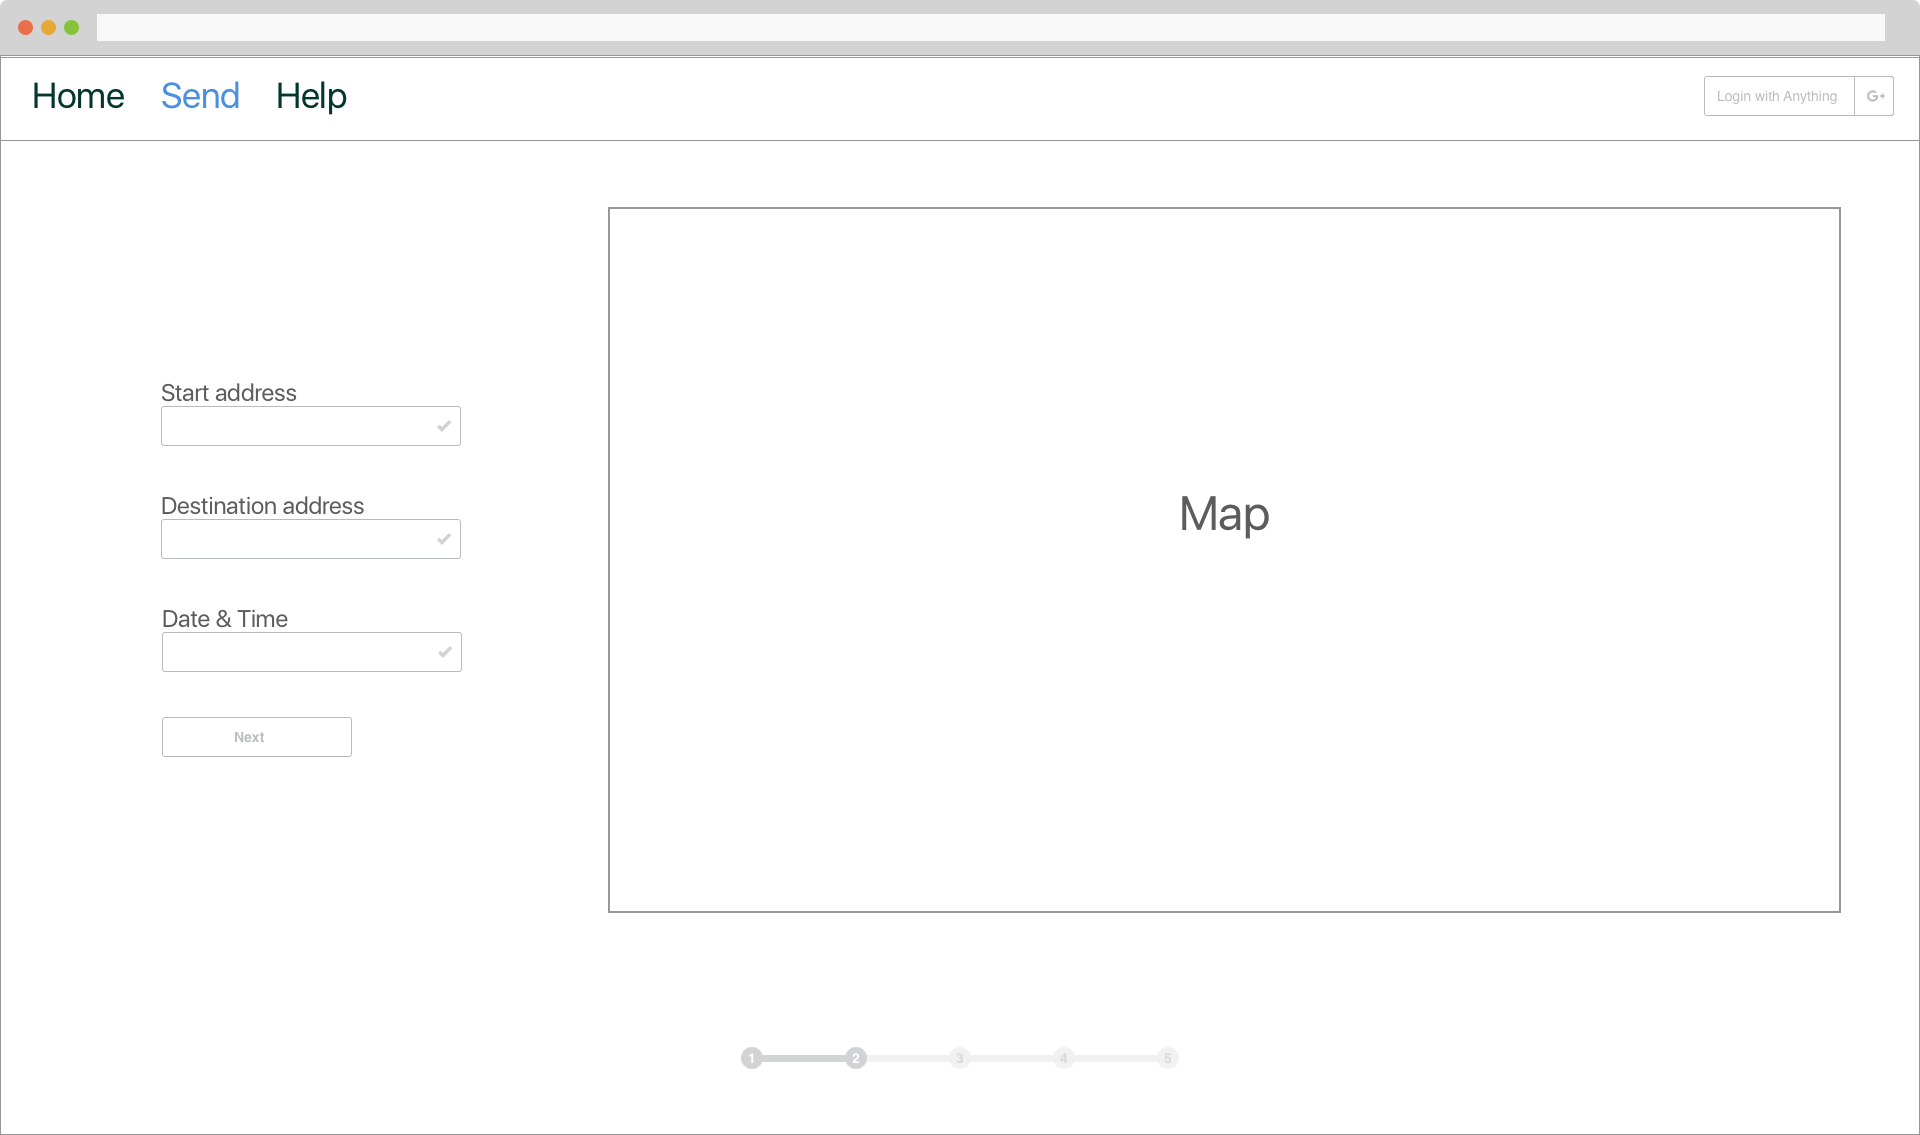
\includegraphics[angle=270,width=0.6\textwidth]{images/step1.png}
  \caption{Wireframe Schritt 1}
  \label{fig:wireframes1}
\end{figure}

\begin{figure}[ht]
  \centering
  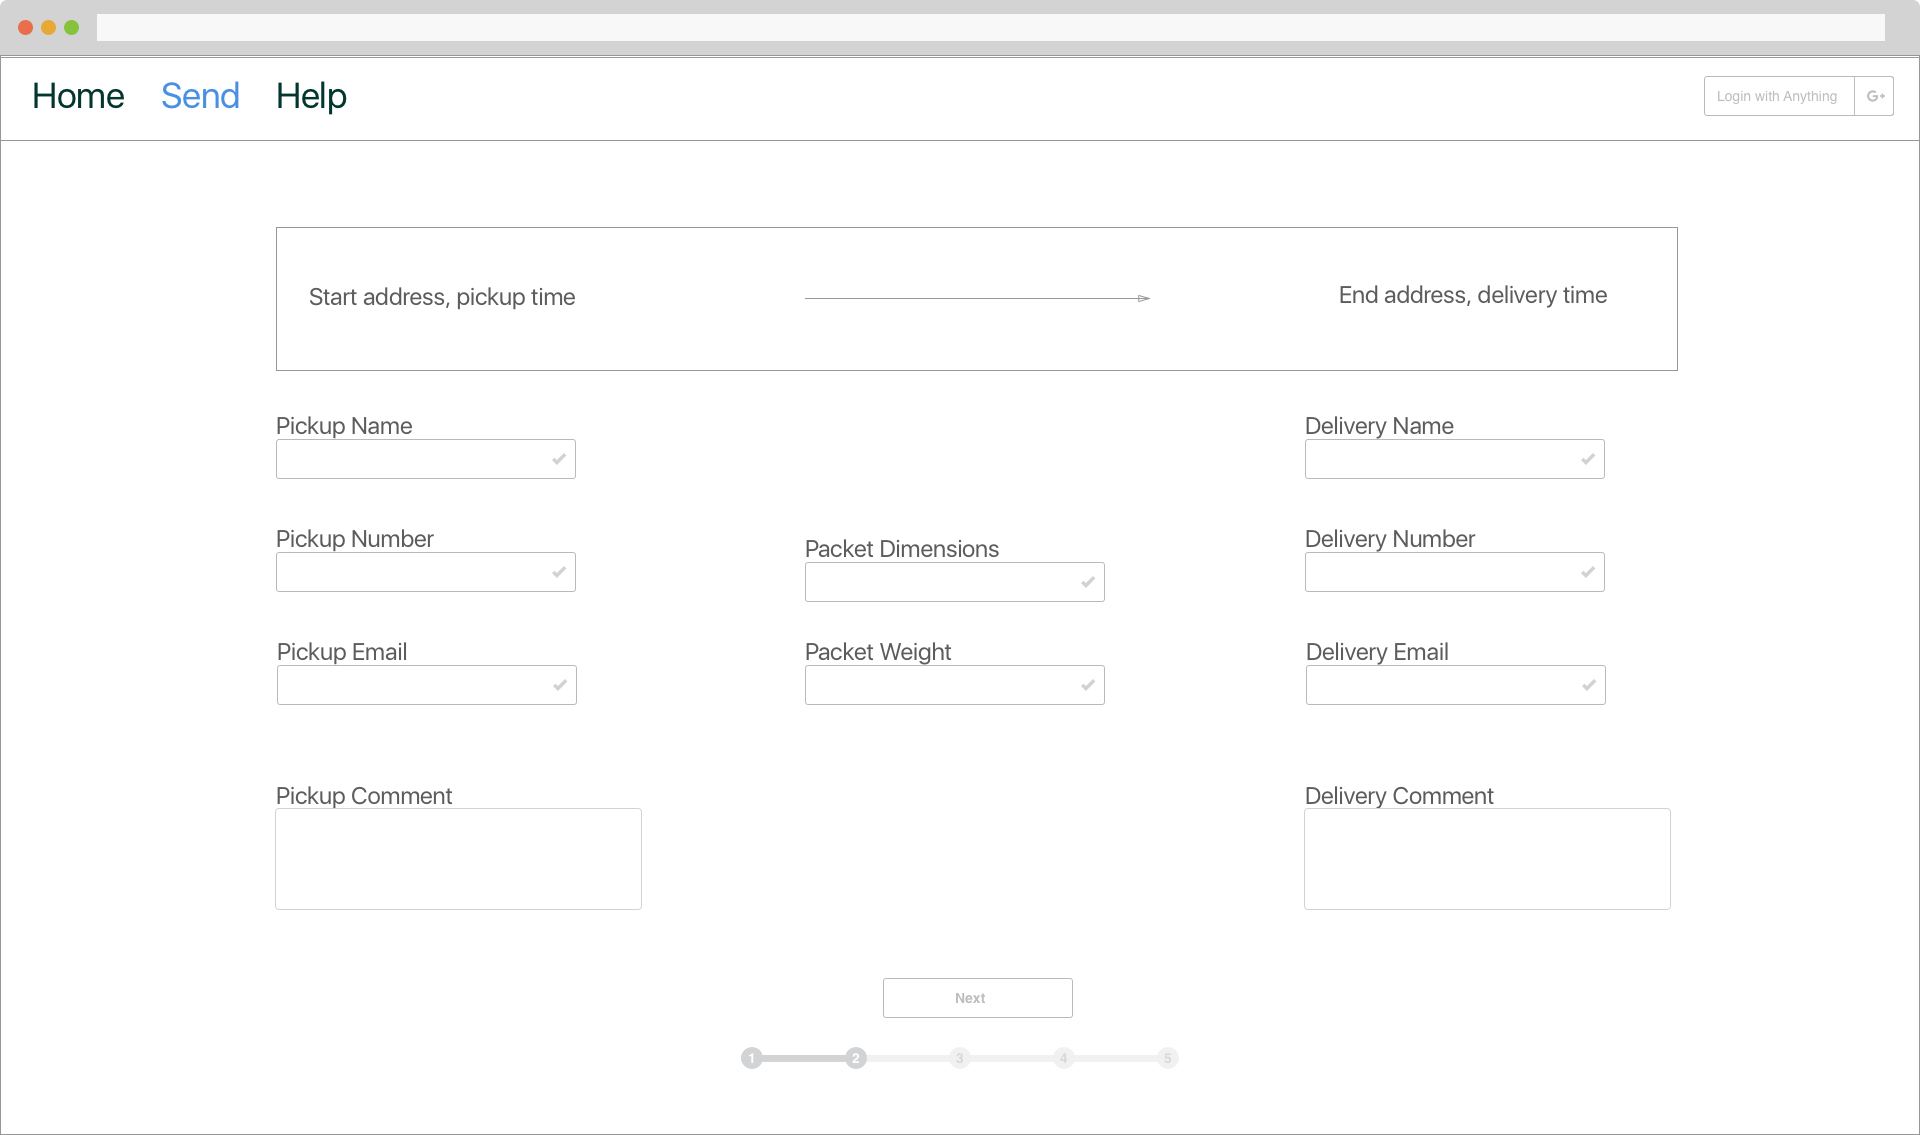
\includegraphics[angle=270,width=0.7\textwidth]{images/step2.png}
  \caption{Wireframe Schritt 2}
  \label{fig:wireframes2}
\end{figure}

\begin{figure}[ht]
  \centering
  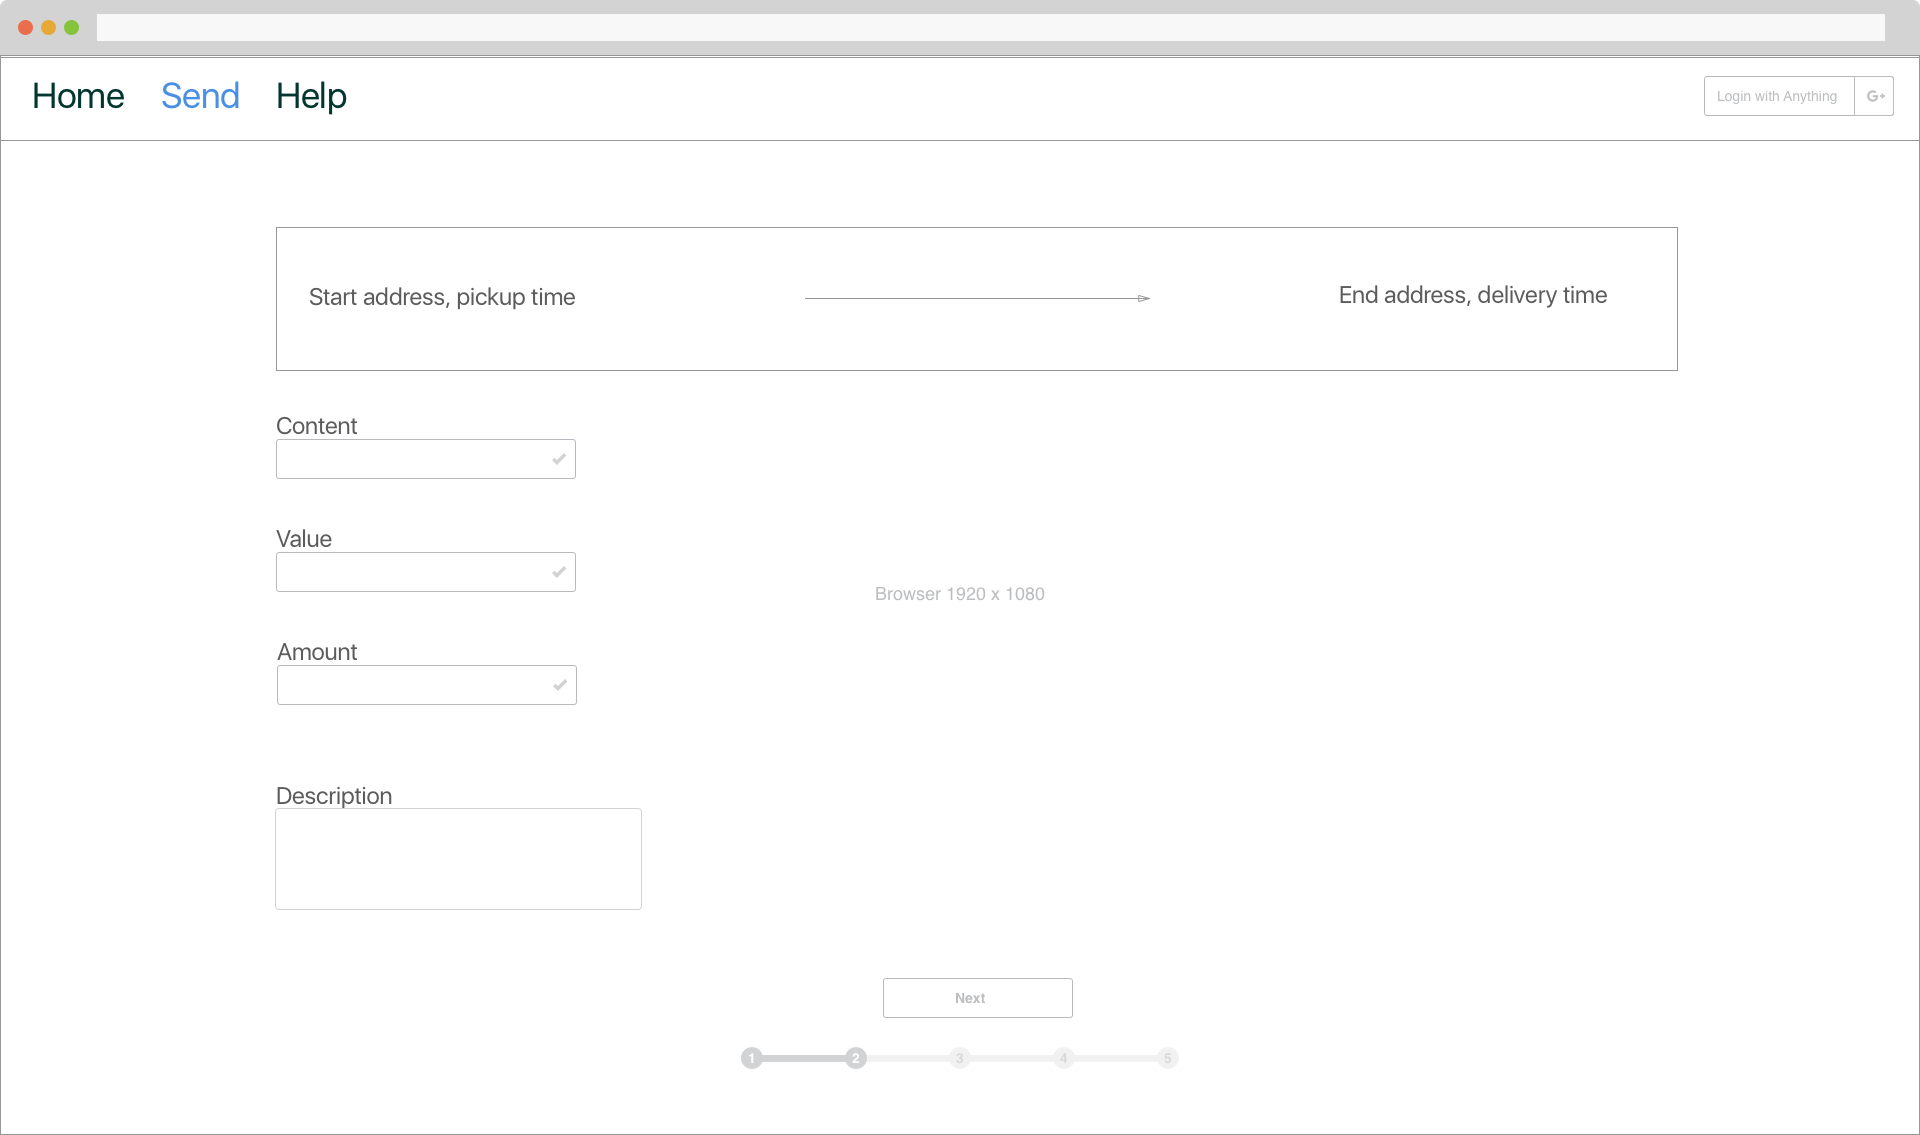
\includegraphics[angle=270,width=0.7\textwidth]{images/step3.png}
  \caption{Wireframe Schritt 3}
  \label{fig:wireframes3}
\end{figure}

\begin{figure}[ht]
  \centering
  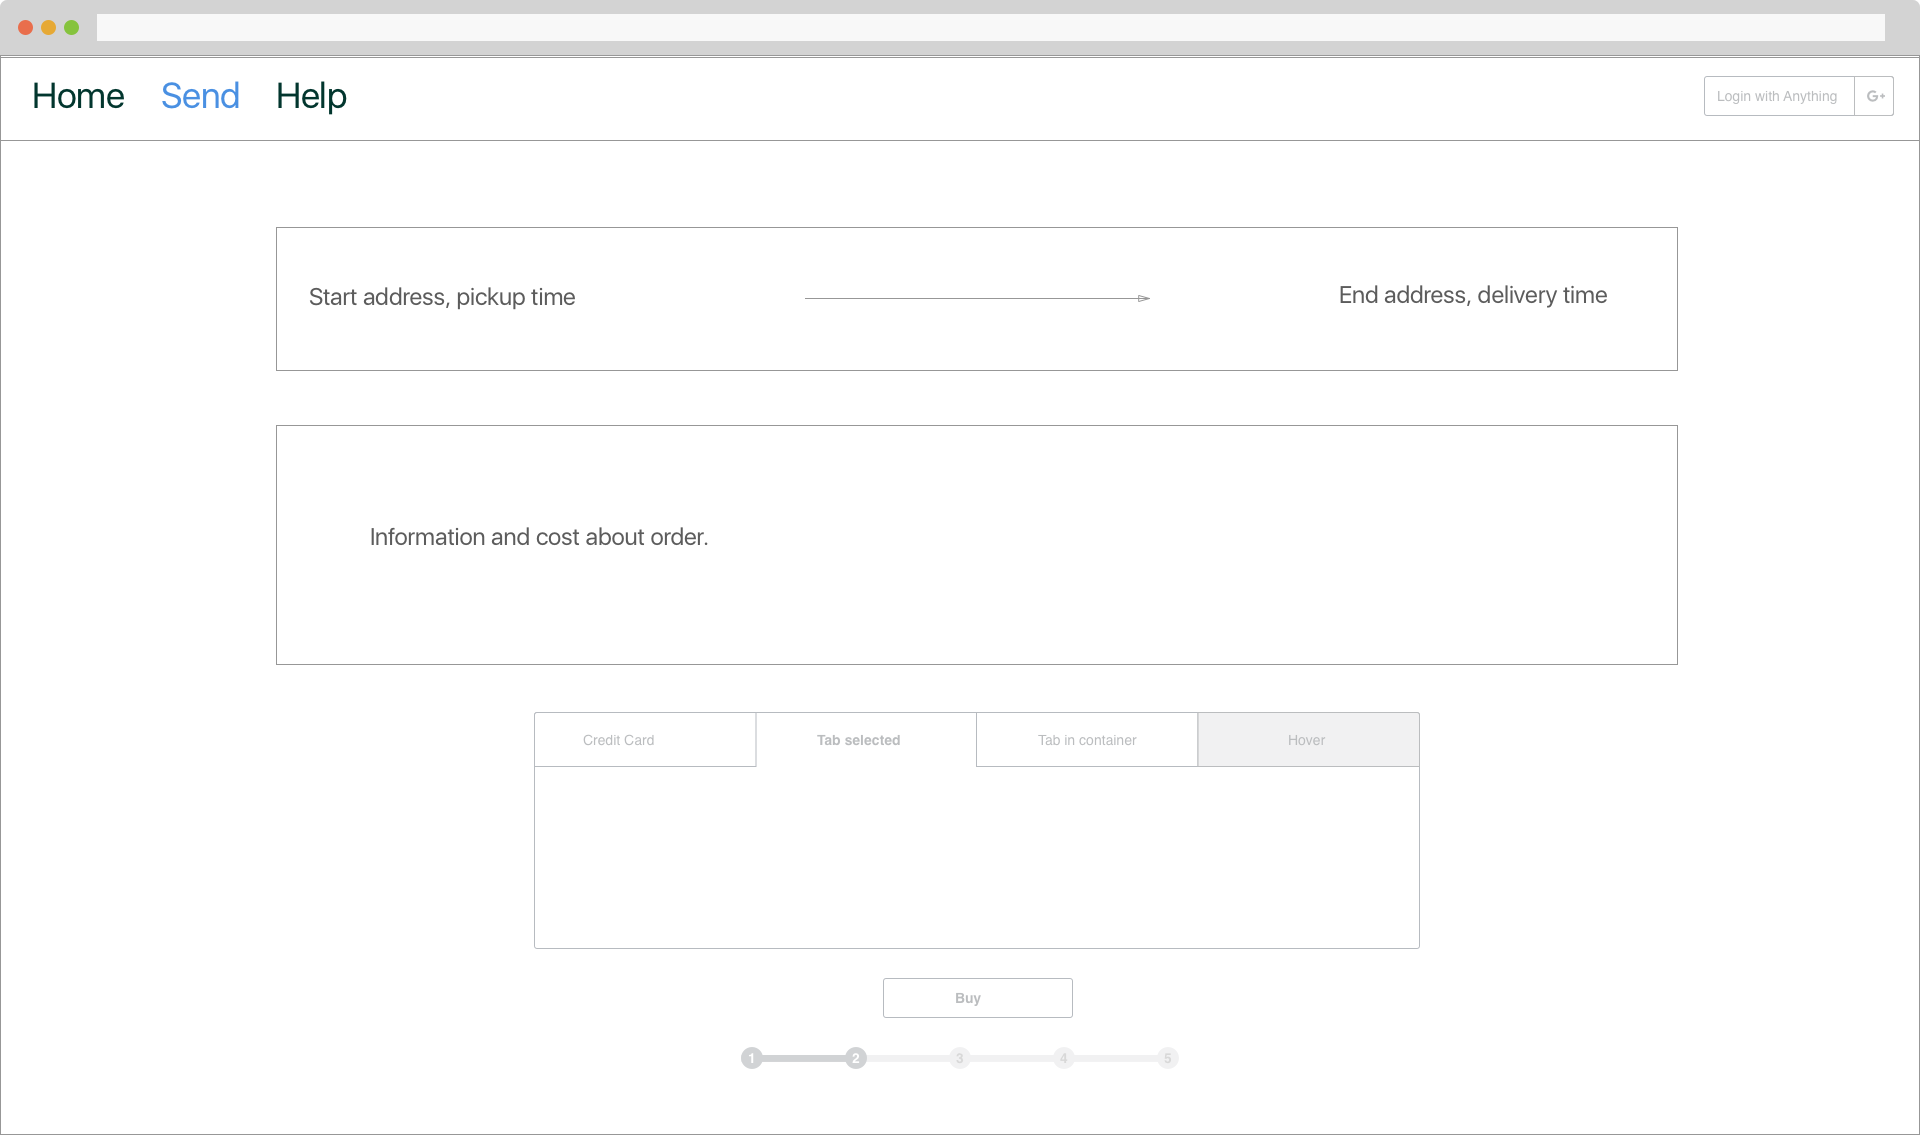
\includegraphics[angle=270,width=0.7\textwidth]{images/step4.png}
  \caption{Wireframe Schritt 4}
  \label{fig:wireframes4}
\end{figure}

\begin{figure}[ht]
  \centering
  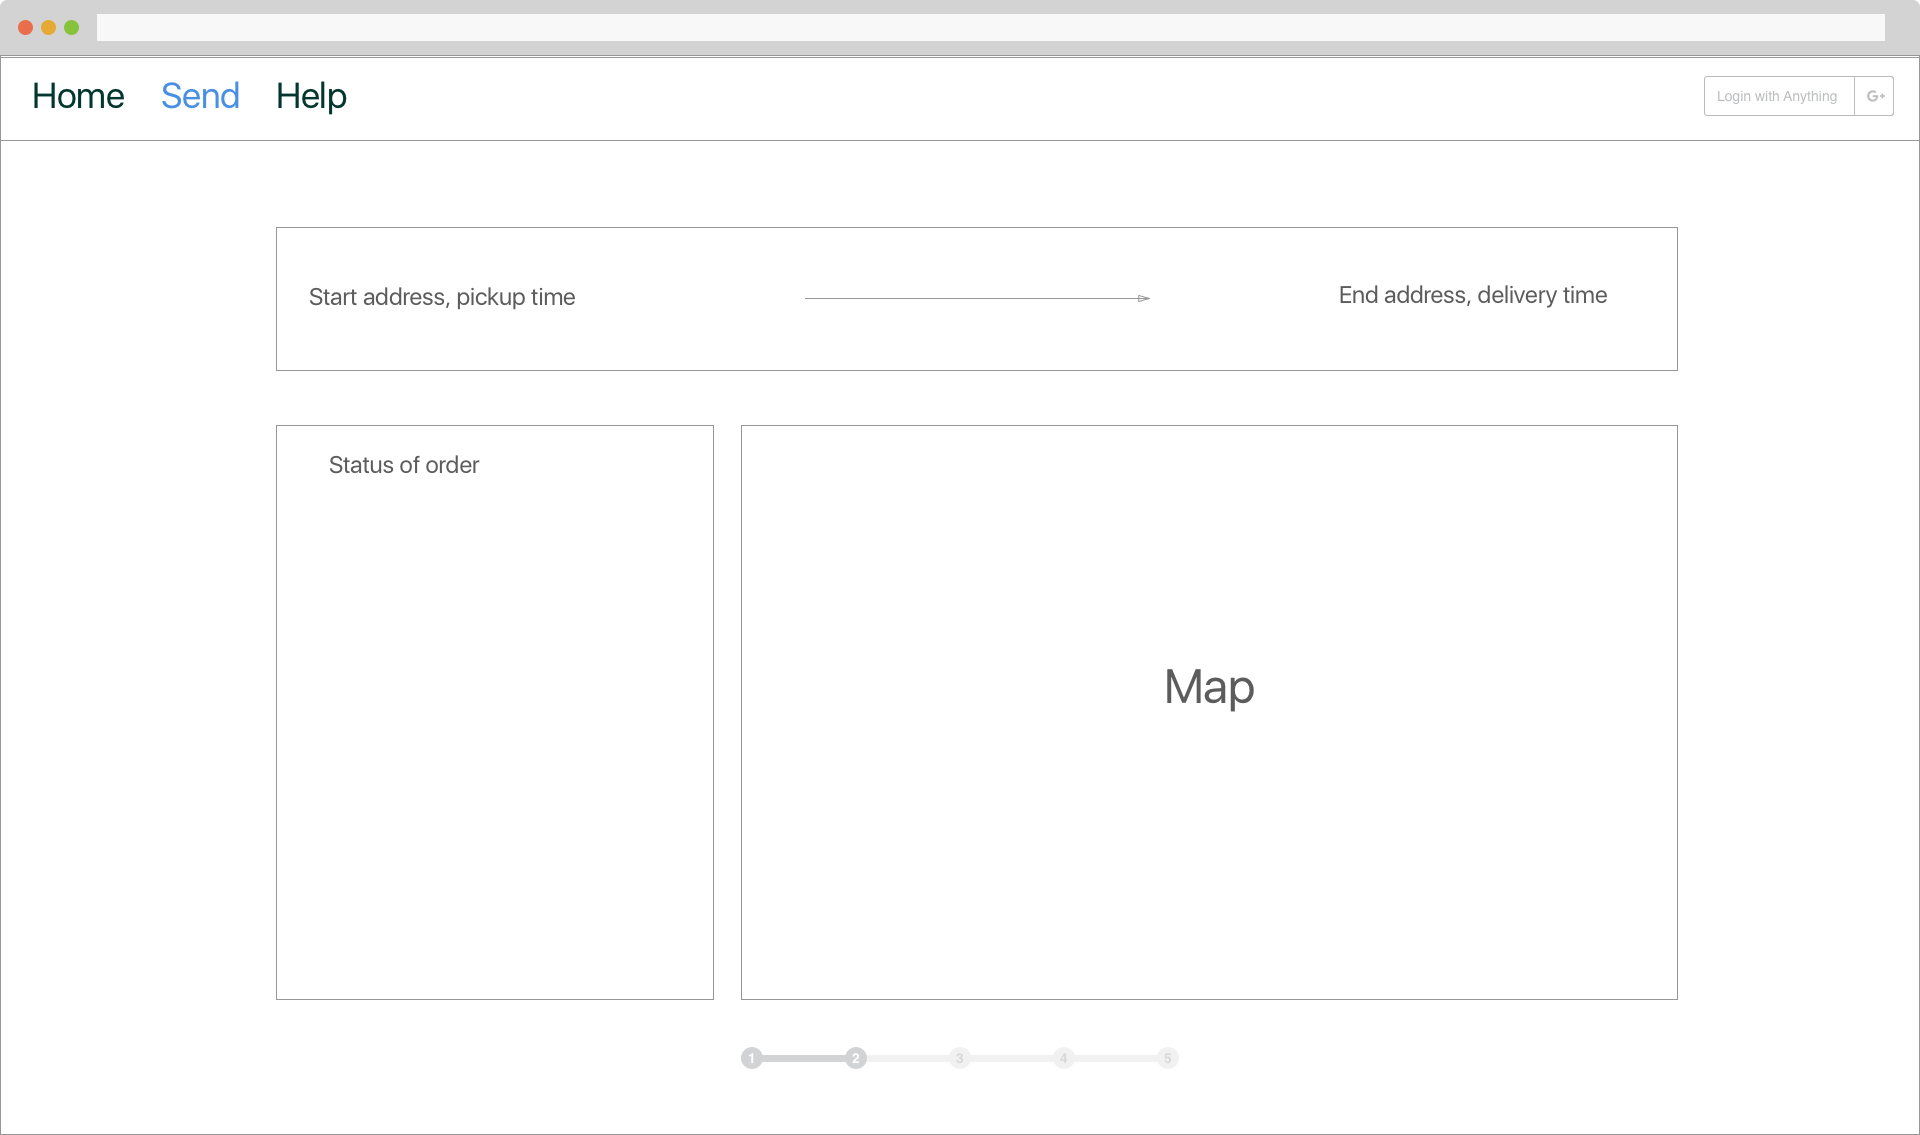
\includegraphics[angle=270,width=0.7\textwidth]{images/step5.png}
  \caption{Wireframe Schritt 5}
  \label{fig:wireframes5}
\end{figure}
